%!TEX root = ../report.tex

\chapter{Contextualization}
\label{chap:chap3}

\section*{}

The primal objective of this dissertation, as referred in chapter \ref{chap:intro}, is to develop one or more software modules that will improve Spotify Users' music discovery and recommendation experience using visual tools to represent the music artists' relations and Spotify's streaming service to provide high quality music stream.

The initial proposal was to develop a module that implements, at least, one of the following features:

\begin{enumerate}
  \label{chap3:modules}
  \item \label{item:obj1} Integrate Spotify's music stream into RAMA's website
  \item \label{item:obj2} Integrate information from the Spotify user into RAMA
  \item \label{item:obj3} Improve RAMA's features and design
  \item \label{item:obj4} Integrate the RAMA concept into a Spotify Application
  \item \label{item:obj5} Integrate RAMA's playlist generation into a Spotify Application
  \item \label{item:obj6} Integrate some of the above mentioned modules into a Mobile Application
\end{enumerate}

The first three functionalities (\ref{item:obj1}, \ref{item:obj2} and \ref{item:obj3}) focus on improving RAMA using Spotify's API, i.e. to integrate Spotify into RAMA.
Whereas \ref{item:obj4} and \ref{item:obj5} aim to integrate RAMA's concept into Spotify, through a Spotify Application (it would work as a plugin to Spotify's Desktop Client).
The last one (\ref{item:obj6}) would focus on implementing the previous functionalities into an Android, iOS or Windows Phone Application.
The aim of this chapter is to compare and contrast these proposed features, towards determining which among them will be pursued in this thesis, either: Spotify Application, Mobile Application, or RAMA improvements.

At first, Spotify's user environment will be introduced (\ref{sec:spotify}), followed by Spotify's Development Tools (\ref{sec:devtools}) in order to assess which tools are available for developers.
Next, the available tools will be evaluated, through experiments (\ref{sec:experiments}), in order to determine which ones fit the proposed modules better.

By the end of this chapter the modules developed should be clearly stated, as well as which development tools will be used in the prototype.
The prototype should pursue the objective of contributing to an improved user experience of discovering new music by taking advantage of visual tools that implement RAMA's concept.

\section{Introducing Spotify} % (fold)
\label{sec:spotify}

  % 

  Spotify is a Music Streaming Service that allows the user, through an Internet connection, to listen to any track (if available in the user's country) in Spotify's catalogue.
  The service was launched in 2008 with a native desktop client application.
  Now, the service has several types of clients available to the users: desktop client, webplayer and mobile applications.

  \begin{description}
    \item[\textbf{Desktop Client}] Desktop version of Spotify, with Windows and Mac versions (and also a Linux preview version).
    \item[\textbf{Webplayer}] Web version of Spotify. This was released in 2013, although spotify still advises the use of the native application for a better user experience.
    \item[\textbf{Mobile Applications}] The mobile applications are available for Android and iOS devices.
  \end{description}

  % \subsection{Music Discovery Tools} % (fold)
  % \label{sub:discovery_tools}
  
  % browse: groups of playlists
  % activity: social side that shows the user's friends' activity on spotify (what they listen to)
  % discover: artists/albums/tracks suggestions based on the user's listening history.
  % top lists: 2


  % subsection discovery_tools (end)


  \section{Development Tools} % (fold)
  \label{sec:devtools}
  
    Spotify provides a set of tools\footnote{\url{http://developer.spotify.com/technologies}} to develop Third-party Applications (websites, native applications and mobile applications) and Spotify Applications (that run inside Spotify's Desktop Client).
    There are five tools, each with different purposes.

    \subsection{Spotify Apps} % (fold)
    \label{sub:spotify_apps}
      Spotify Applications~\cite{spotifyapps} are a special case in the whole set of tools provided by Spotify.
      These applications are designed to run \emph{inside} the Desktop Client.
      Spotify users can run and install applications from the store called "App Finder".
      All the applications are free.
      In Figure~\ref{fig:spotify_apps} one can see the interface of the desktop client.
      In this case, the discovery mode's interface.
      \begin{figure}
        \begin{center}
          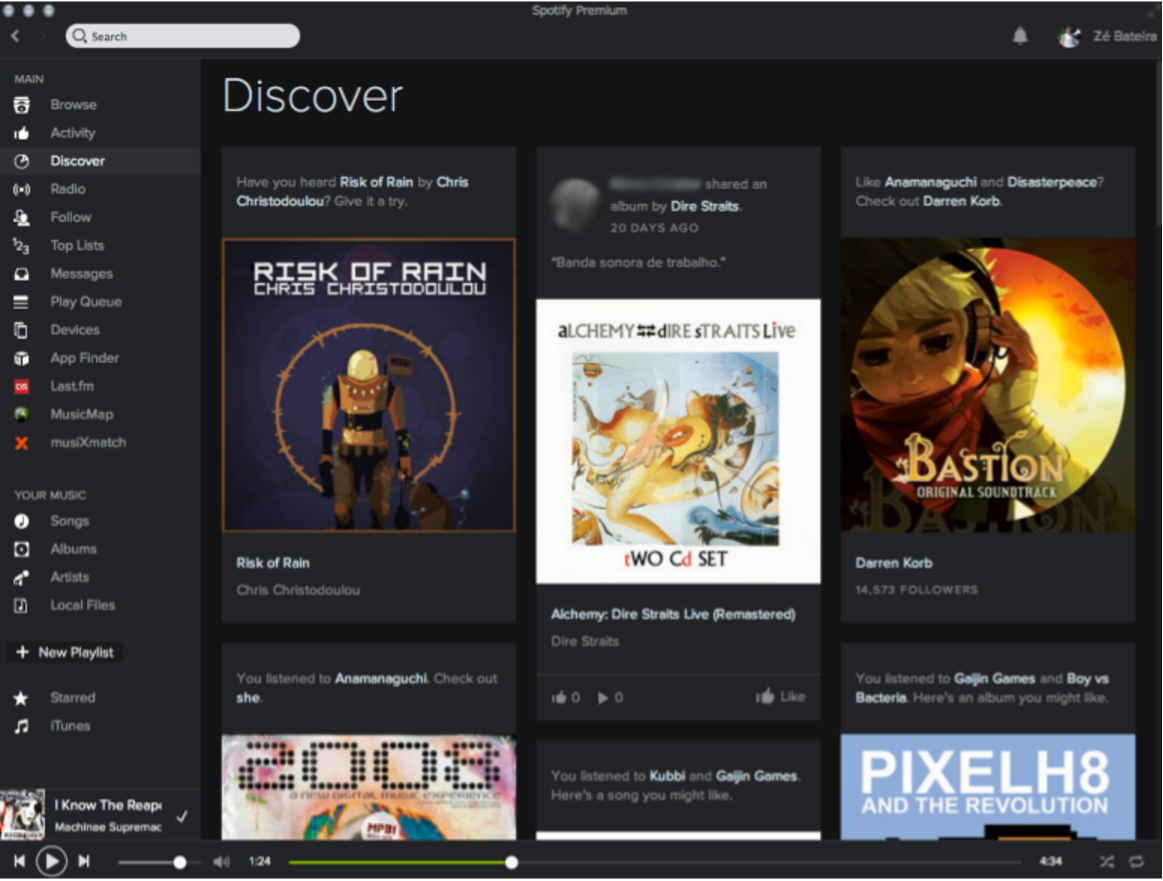
\includegraphics[width=\textwidth]{spotify_discovery.mode.pdf}
        \end{center}
        \caption{Spotify: desktop client's discovery mode interface.}
        \label{fig:spotify_apps}
      \end{figure}
      On the left side, in the menu, bellow the "App Finder" item, appears all the applications the user as installed from the store.
      In Figure~\ref{fig:spotify_apps2} the official Last.fm application is opened.
      Note how the space filled by the applications are always the same.

      \begin{figure}
        \begin{center}
          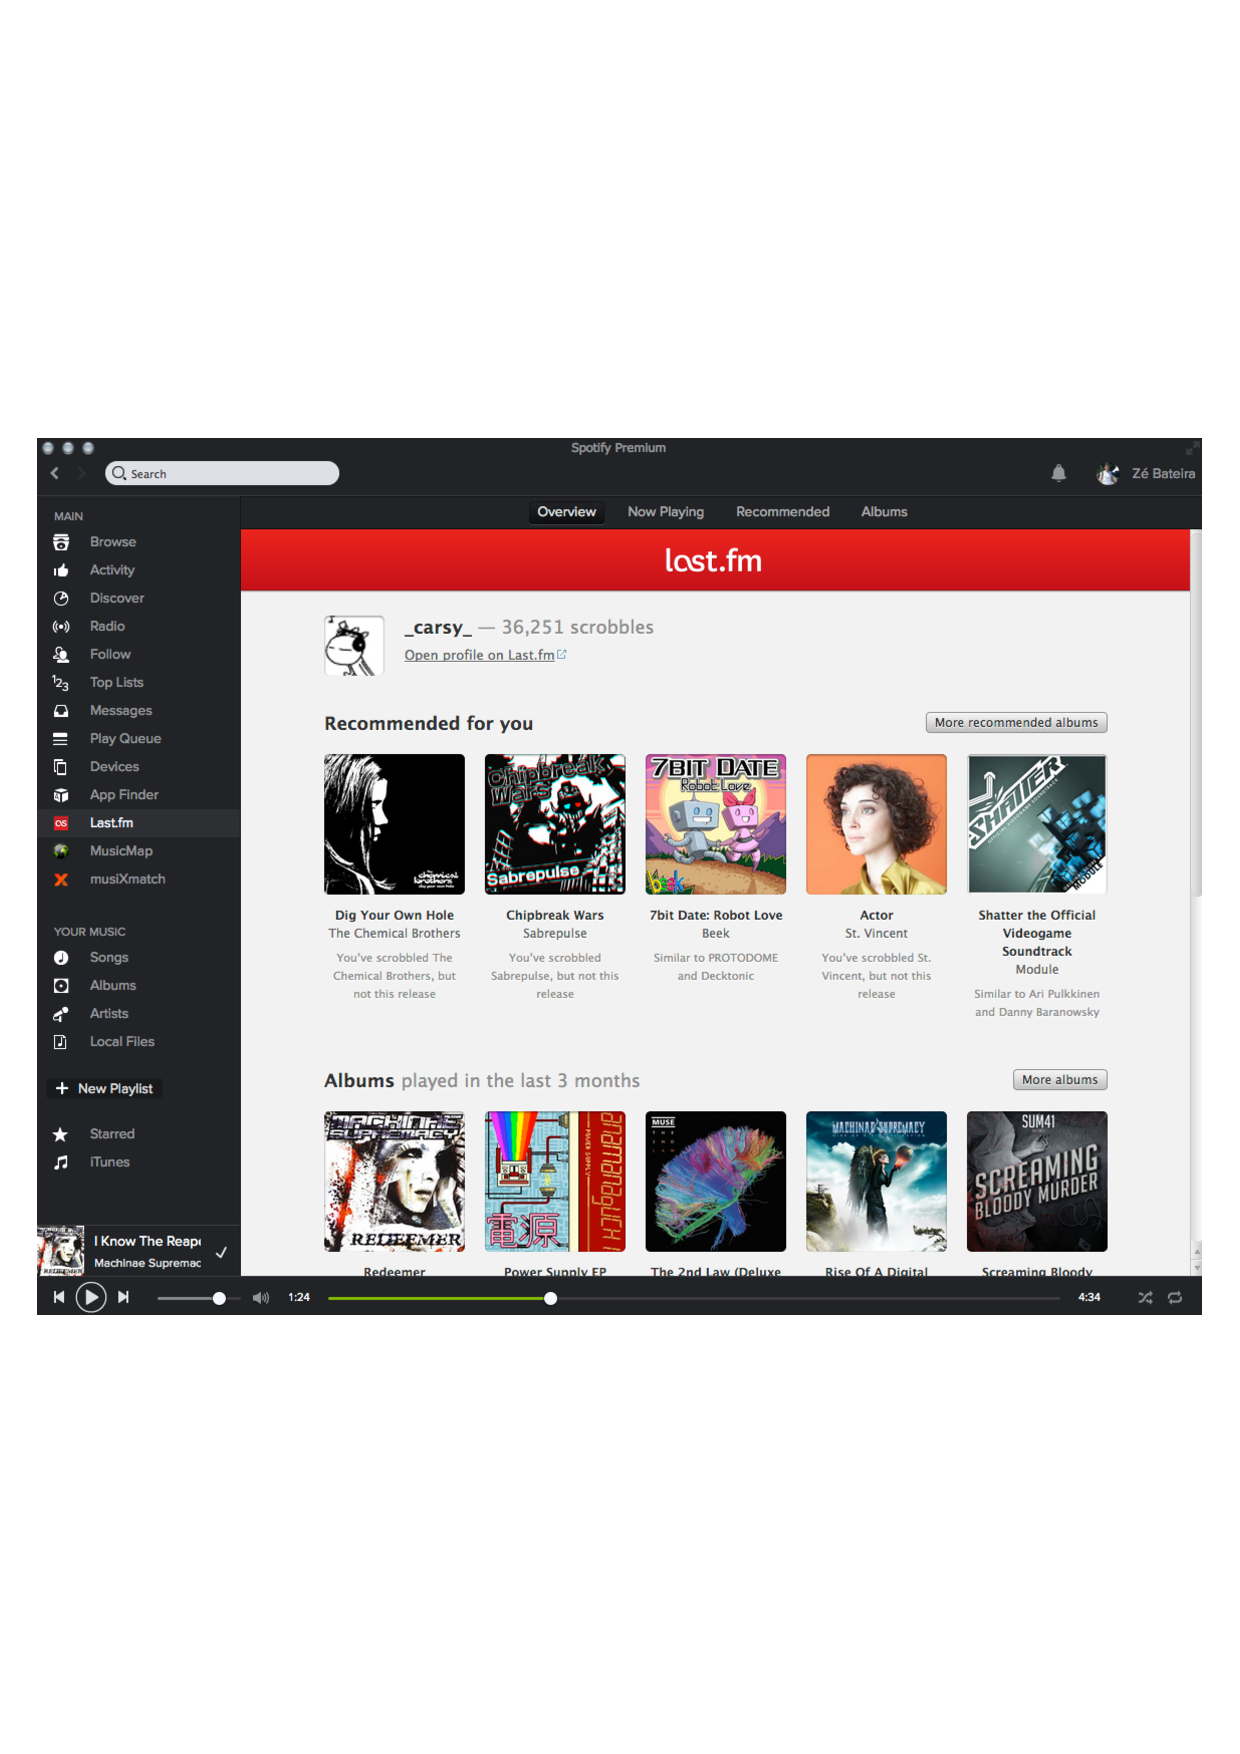
\includegraphics[width=\textwidth]{spotify_apps.pdf}
        \end{center}
        \caption{Spotify: Last.fm's Spotify Application opened.}
        \label{fig:spotify_apps2}
      \end{figure}

      The Applications' runtime environment is one of a browser-based.
      More specifically, powered by the Chromium Embedded Framework~\cite{chromiumembedded}.
      This means that the code to develop a Spotify Application follows the same principles as a web application: HTML, CSS and Javascript.

      Spotify developed two Frameworks\footnote{\url{https://developer.spotify.com/technologies/apps/reference}} to help developers create these applications: the API 1.x Framework\footnote{\url{https://developer.spotify.com/docs/apps/api/1.0/}} and the Views Framework\footnote{\url{https://developer.spotify.com/docs/apps/views/1.0/}}.
      The first one provides an interface to use object models, access metadata, control the player, among others.
      The second offers support for web components like buttons, lists, tabs, among others.

    % subsubsection spotify_apps (end)


    \subsection{Spotify Widgets} % (fold)
    \label{sub:spotify_widgets}

      Spotify Widgets\footnote{\url{https://developer.spotify.com/technologies/widgets}} are small web components that can be embedded in external websites.
      Spotify provides two components: \emph{Play Button} (Figure~\ref{fig:spotify_play_button}) and a \emph{Follow Button} (Figure~\ref{fig:spotify_follow_button})

      \begin{figure}[H]
        \begin{center}
          
\includegraphics[width=0.5\textwidth]{spotify_play_button.pdf}
        \end{center}
        \caption{Spotify: \emph{Play Button}.}
        \label{fig:spotify_play_button}
      \end{figure}

      \begin{figure}[H]
        \begin{center}
          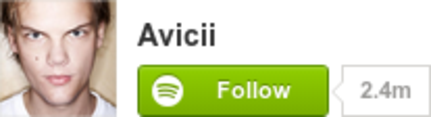
\includegraphics[width=0.5\textwidth]{spotify_follow_button.pdf}
        \end{center}
        \caption{Spotify: \emph{Follow Button} Allows the user to follow the music artist.}
        \label{fig:spotify_follow_button}
      \end{figure}

      However, there are some limitations.
      In Spotify, only logged in users can use the service (listen to tracks, etc).
      This also applies to these widgets - even if they are in an external application, only Spotify users can interact with them.
      This limitation does make sense in the case of the \emph{Follow Button}, but the \emph{Play Button} becomes useless to non-Spotify users.
      In truth, these widgets are nothing but an hyperlink to a Spotify Client (Web Player or Desktop).
      With the Play Button, the stream of tracks always plays inside Spotify's environment, and not on external applications.

      To embed a widget, it is only required to copy-paste Html code into the website, where appropriate:

      \lstinputlisting[language=HTML,caption={Html code to embed the \emph{Play Button}}, style=htmlcssjs, captionpos=b]{snippets/play_button.html}

      These widgets are useful to develop the proposed modules \ref{item:obj1} and \ref{item:obj3}.

    % subsubsection spotify_widgets (end)

    \subsection{Libspotify SDK} % (fold)
    \label{sub:libspotify_sdk}

      Libspotify SDK\footnote{\url{https://developer.spotify.com/technologies/libspotify}} is an API that allows for third-party applications to include Spotify's services into them.
      However, not without some limitations to the users of these applications.
      The users are limited depending on the type of Spotify Subscription that they have signed up to.

      There are three different types of subscriptions, but the important part to retain, is the difference between being a Free Subscription Spotify User, and a Paid Subscription Spotify User (premium and unlimited subscriptions).
      As mentioned before, only Spotify users can interact with Spotify Widgets (Figure~\ref{sub:spotify_widgets}).
      That also applies to third-party applications that are using Libspotify SDK, which allow, for example, the user to login with their Spotify account.
      But in this case, not only do they need to be Spotify users, they also need to have signed up to a paid Spotify subscription.
      And not only do the users need to pay to use the Spotify-powered application, but the developers as well.
      This is a very restrictive environment, although Libspotify SDK comes in many different flavours~\cite{libspotifysdk}.

      This tool would be used to develop modules \ref{item:obj1}, \ref{item:obj2} and \ref{item:obj6}.
      

    % subsubsection libspotify_sdk (end)


    \subsection{Metadata API} % (fold)
    \label{sub:metadata_api}

      The \emph{Metadata API}\footnote{Metadata API: \url{https://developer.spotify.com/technologies/web-api}. This API was recently deprecated (June, 2014) and was replaced by the \emph{Web API}. It follows the same principles of the previous one, and so, for the purposes of this report, the differences are not relevant.} allows for applications to retrieve information from Spotify's music catalogue: tracks, albums, artists, playlists, and so on.

      Requests to the database are done through HTTP and are of two types: \emph{search}\footnote{\url{https://developer.spotify.com/technologies/web-api/search}} e \emph{lookup}\footnote{\url{https://developer.spotify.com/technologies/web-api/lookup}}.
      To request detailed information of, e.g., an artist, the URI (used as the unique identifier) of that artist is required. Such ID is of the form:

      \url{spotify:artist:<artist_id>}, where \emph{artist\_id} is the unique identifier of the artist.

      Example:

      \url{spotify:artist:65nZq8l5VZRG4X445F5kmN}, is the ID for the artist "Mariza". \\

      There's also ID's for albums:

      \url{spotify:album:5d1LpIPmTTrvPltx26TlEU} (album "Fado Tradicional" from "Mariza") \\

       and for tracks:

       \url{spotify:track:2vqYasauhDLVjTt7CGWK6y} (track "Fado Vianinha" of the previous album) \\

      These URI schemes are compliant with Rosetta Stone's ID spaces~\cite{rosettastone}.

      First, to get this URI, one needs to search the database.

      \begin{description}
        \item[\emph{Search}] \hfill

          The base \emph{URL}:

          \url{http://ws.spotify.com/search/1/album}, to search for albums.

          For artists, \emph{artist}, for tracks, \emph{track}. \\

          Examples:

          \url{http://ws.spotify.com/search/1/album?q=foo} \\
          \url{http://ws.spotify.com/search/1/artist.json?q=red+hot} \\

          The request response, by default, is formatted in \emph{XML}, although, as the second example demonstrates, \emph{JSON} is also supported.

          Given the following query: \\
          \url{http://ws.spotify.com/search/1/artist.json?q=camane}

          The server responds with:

          \lstinputlisting[caption={Results ordered by "popularity"}, style=htmlcssjs, captionpos=b]{snippets/search_camane.json}

        \item[\emph{Lookup}] \hfill \\

          When the URI is known, one can finally lookup detailed information about a database item. With the following query:

          \sloppy
          \url{http://ws.spotify.com/lookup/1/.json?uri=spotify:artist:3MLPFTe4BrpEV2eOVG0gLK&extras=album}

          The server responds with:

          \lstinputlisting[caption={\emph{lookup} of the artist "Camané"}, style=htmlcssjs, captionpos=b]{snippets/lookup_camane.json}

      \end{description}

      This API is very useful for all the six proposed modules.

    % subsubsection metadata_api (end)

    \subsection{iOS SDK (beta)} % (fold)
    \label{sub:ios_sdk}
    
    The iOS SDK supports iOS Application developers. Although still in beta\footnote{\url{https://developer.spotify.com/technologies/spotify-ios-sdk}}, this tool would be used to develop the proposed module \ref{item:obj6}.
    Much like the Libspotify SDK, this SDK provides the following APIs:

    \begin{itemize}
      \item User authentication
      \item Audio playback and stream management
      \item Metadata (artist, album, track) lookup including artwork
      \item Playlist management
    \end{itemize}

    % subsubsection ios_sdk (end)

  % subsection devtools (end)

  \section{Experiments} % (fold)
  \label{sec:experiments}

    As a first hands-on experience with these tools, a single-page website was developed which allows the users to search and listen to music using Spotify's \emph{Metadata API} and \emph{Widgets}: \\

    \url{http://carsy.github.io/spotify-playground} \\

    In Figure~\ref{fig:playground} one can see a search result and the \emph{Widget Play Button} with the selected item.

    \begin{figure}
      \centering

      \begin{subfigure}{0.38\textwidth}
        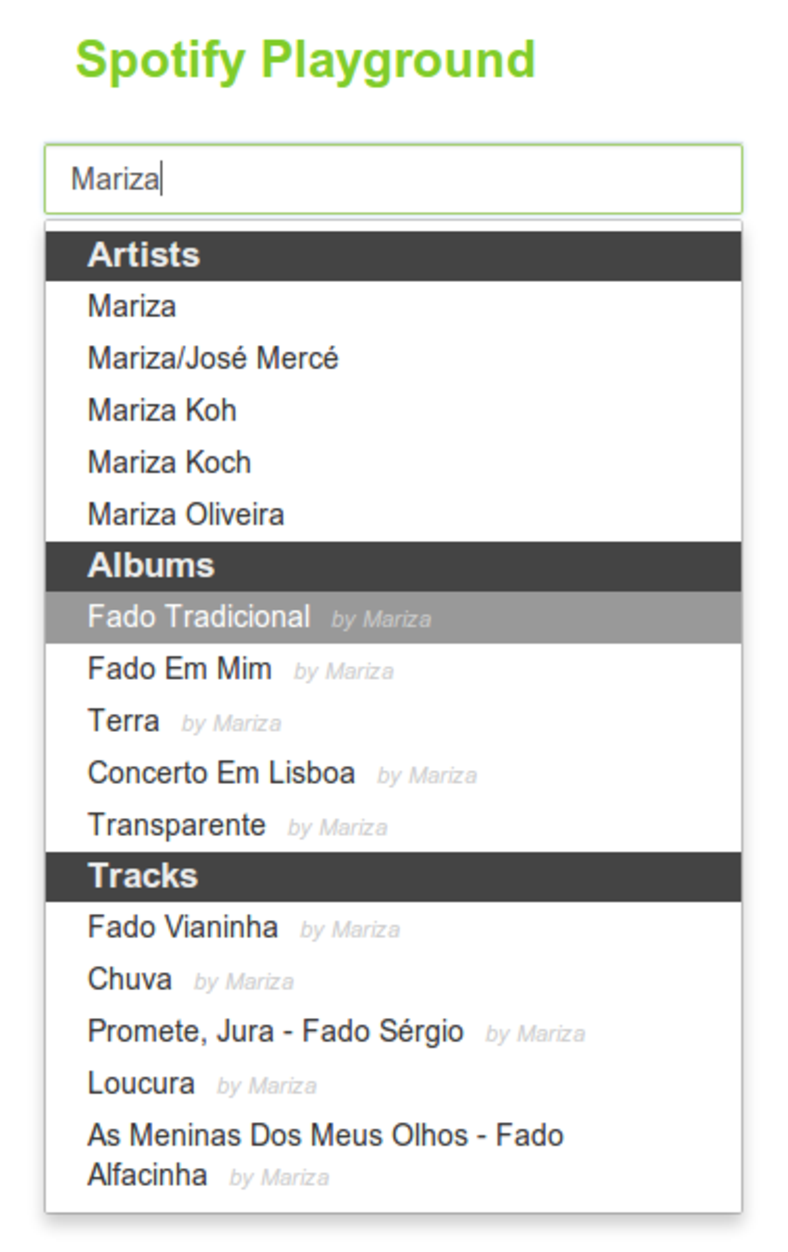
\includegraphics[width=\textwidth]{playground.pdf}
        \caption{Search result for "Mariza"}
        \label{fig:playgroun_a}
      \end{subfigure}

      \begin{subfigure}{0.38\textwidth}
        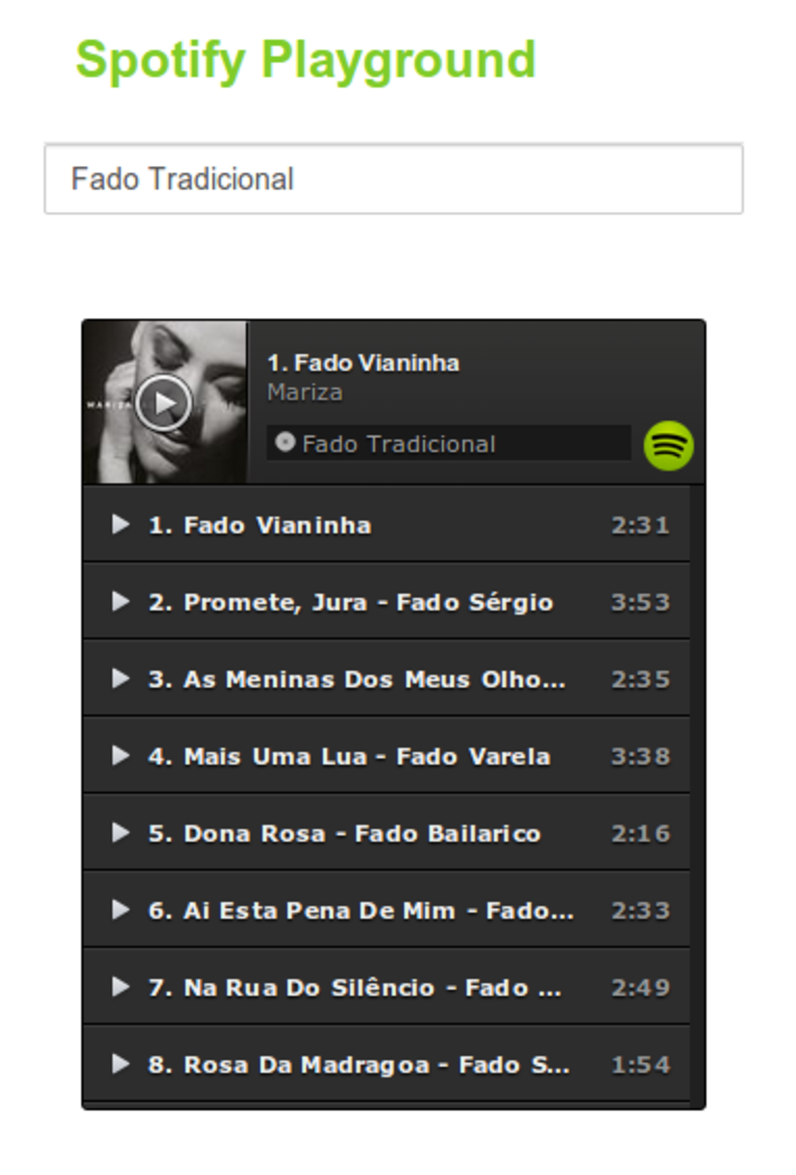
\includegraphics[width=\textwidth]{playground2.pdf}
        \caption{After selecting the album "Fado Tradicional" the \emph{Play button} displays all of the album's tracks to be played in sequence.}
        \label{fig:playground_b}
      \end{subfigure}

      \caption{Experiment with the \emph{Metadata API} and the \emph{Play Button Widget} (source code: \url{github.com/carsy/spotify-playground})}
      \label{fig:playground}

    \end{figure}

    Both tools turned out to be well documented and easy to use.

    Another experiment was made in order to assert the potential of Spotify Applications.
    There was a need to know if the canvas element was well supported by Spotify's environment, because that is the preferred way to graphically draw a graph.
    To test that, a simple application was created with the following code:

    \begin{lstlisting}[caption={\emph{iframe} element that allows to embed RAMA's website into the application.}, style=htmlcssjs, captionpos=b]
      <iframe src="http://rama.inescporto.pt/app" frameborder="0">
      </iframe>\end{lstlisting}

    The final result can be seen in Figure~\ref{fig:rama_spotifyed}.
    \begin{figure}
      \begin{center}
        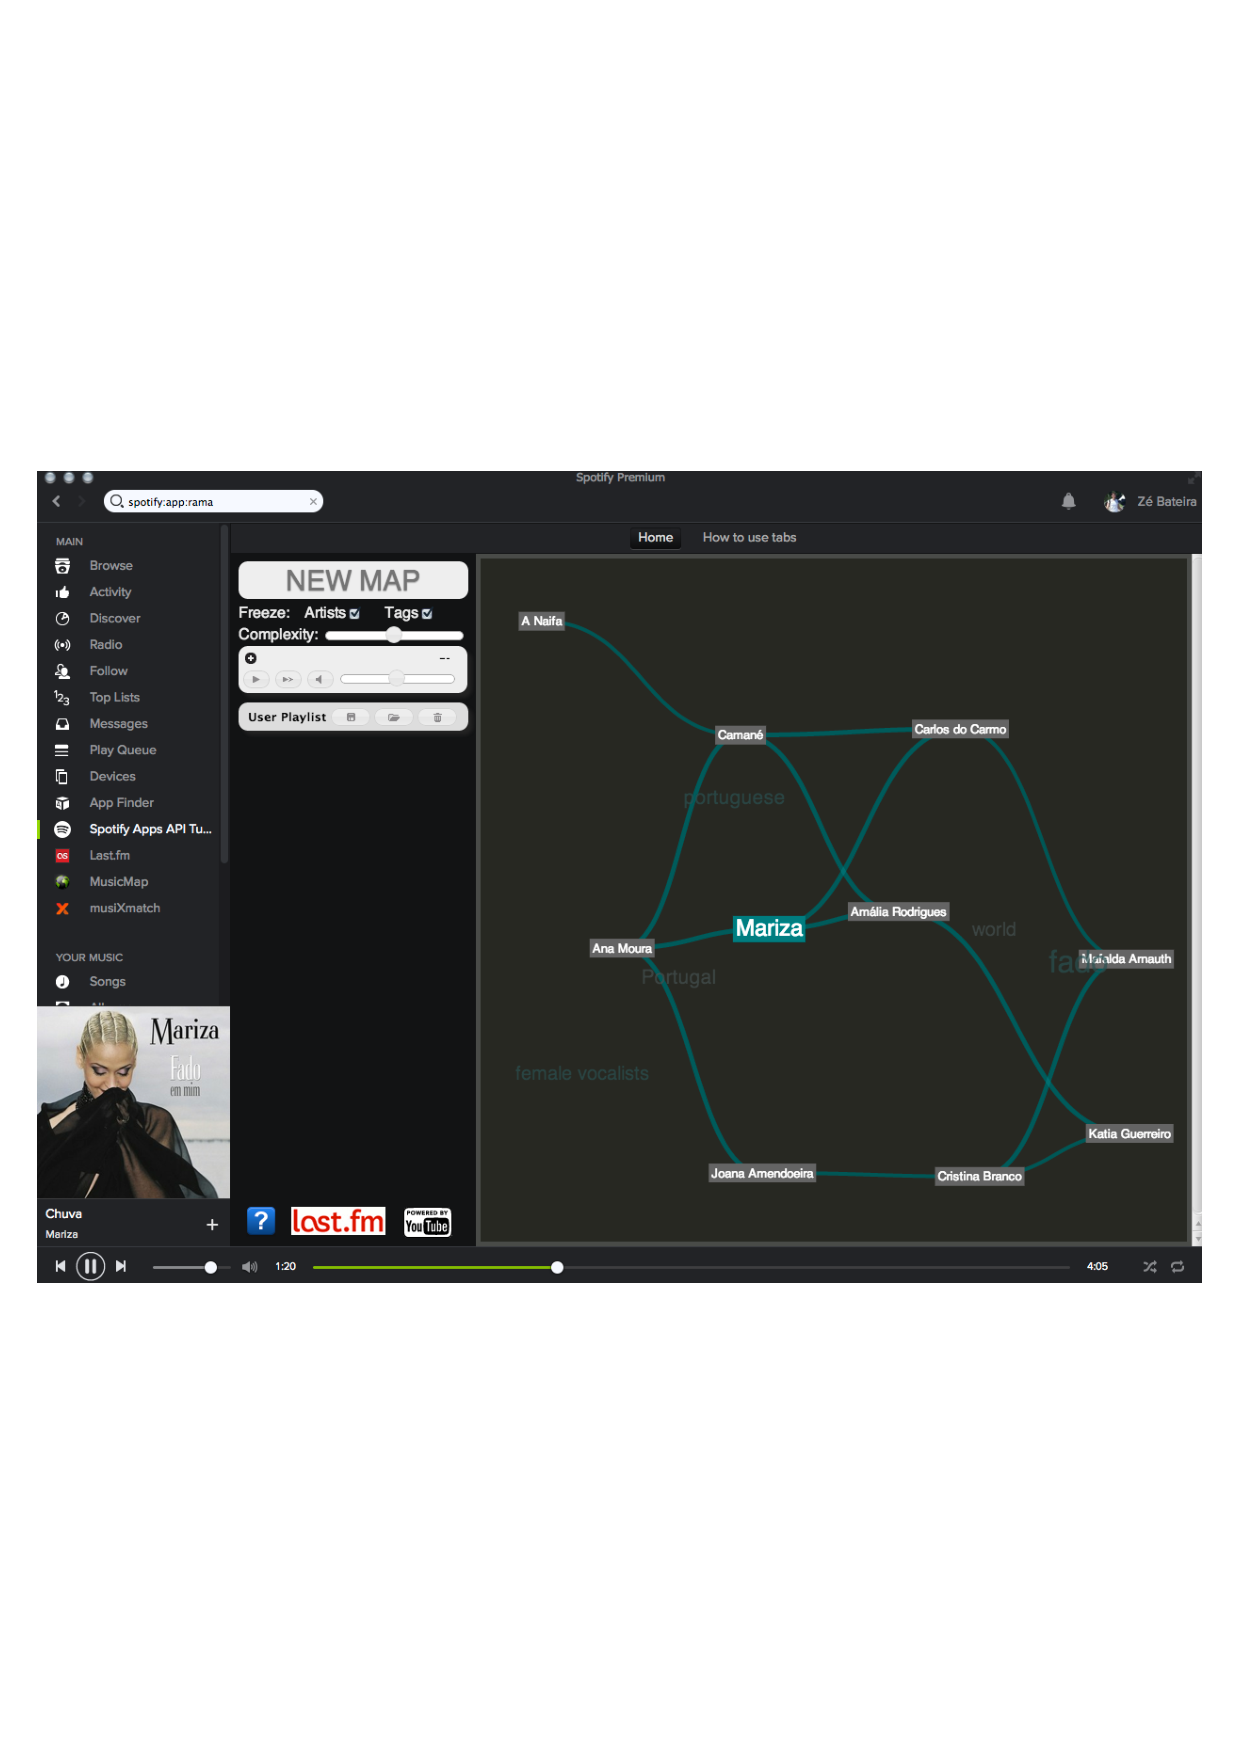
\includegraphics[width=\textwidth]{spotify_rama.embedded.pdf}
      \end{center}
      \caption{RAMA's website embedded into a Spotify Application.}
      \label{fig:rama_spotifyed}
    \end{figure}
    Although the \emph{iframe} and \emph{canvas} elements are supported, there are some that are not.
    This specific application is not usable since, for example, playing tracks from external sources is not allowed.
    Nonetheless, there is a way to test which Html elements are supported, using an internal Spotify application.
    In Figure~\ref{fig:canvas_support} one can see the 100\% supported canvas element.

    \begin{figure}[H]
       \begin{center}
         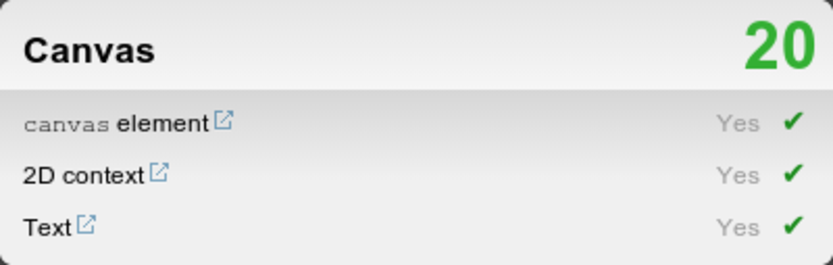
\includegraphics[width=0.5\textwidth]{canvas_support.pdf}
       \end{center}
       \caption{Test result for the canvas element.}
       \label{fig:canvas_support}
     \end{figure}

  % subsection experiments (end)

% section spotify (end)

\section{Summary}

  Based on the analysis conducted, the most appropriate solution was to develop a Spotify Application.
  Although the other proposals were also feasible, the possibility to integrate a RAMA-like interface into Spotify's Desktop Client leaves a Spotify User more at ease with the environment.
  The prototype should then implement the proposed modules \ref{item:obj4} and \ref{item:obj5}:

  \begin{itemize}
    \item[4.] Integrate the RAMA concept into a Spotify Application
    \item[5.] Integrate RAMA's playlist generation into a Spotify Application
  \end{itemize}
